\section{Die Algorithmen auf diesem Markt}
Der Vergleich der RL-Algorithmen findet auf dem in \ref{section:markov} definierten Markt statt.
Dieser Markt wird auf der Testplattform simuliert, die im Rahmen des Bachelorprojektes entwickelt wurde.
Mit den Agenten wird über die Gym-Schnittstelle kommuniziert. \cite{brockman2016openai}
Für die zu vergleichenden Algorithmen werden die Implementierungen der Bibliothek \textit{Stable Baselines} verwendet. \cite{stable-baselines}
Stable Baselines ist eine weit verbreitete eine Open-Source RL-Bibliothek, die in Python geschrieben ist.
Sie baut auf PyTorch auf, einem der beliebtesten Deep-Learning-Frameworks, das in der Forschung weite Verbreitung findet. \cite{NEURIPS2019_9015}
Die in Stable Baselines implementierten Algorithmen entsprechen in den meisten Fällen unmittelbar den vorgeschlagenen Algorithmen der Originalpaper und zeichnen sich durch eine hohe Lesbarkeit des Codes aus.
Alle Hyperparameter sind konfigurierbar.

In dieser Untersuchung der Algorithmen wird stets von den Hyperparametern der Originalpaper ausgegangen.
Diese sind auch im Abschnitt \ref{section:hyperparameter} zu finden.
Weil kaum theoretische Erkenntnisse über die Ermittlung optimaler Hyperparameter vorliegen und diese stets problemspezifisch sind, ist eine erschöpfende Optimierung der Hyperparameter nur mit erheblichem experimentellem Aufwand möglich.
Dazu müssten sehr viele Kombinationen mit jeweils mehreren Läufen durchgeführt werden, was einen nicht zu leistenden Ressourcenaufwand darstellt.
Dennoch wurden an einigen Stellen bessere Hyperparameter gefunden und Aussagen über die Algorithmen über mehrere Hyperparameterkombinationen abgesichert.

Alle Verfahren werden mit neuronalen Netzen durchgeführt, die zwei versteckte Schichten mit je 64 Neuronen haben.
Das Verhalten der Algorithmen für unterschiedliche Netzgrößen ist aber sehr ähnlich, wie die Experimente mit unterschiedlichen Netzgrößen im Bereich [noch zu erstellen] des Anhangs zeigen.
Zunächst werden alle Algorithmen im Duopol gegen den regelbasierten, unterbietenden Wettbewerber aus Abschnitt \ref{section:rulebased_definition} trainiert und evaluiert.
Anschließend werden Training gegen die eigene Policy, unvollständige Informationen, angepasste Rewardfunktion und Monopol- und Oligopolszenarien untersucht.

\section{DDPG und TD3}
\label{section:main_ddpg}
Bei der Diskussion der Q-Learning-Verfahren beschränkt sich diese Analyse direkt auf die Verfahren, die im stetigen Raum angewendet werden: DDPG und TD3.
Diese Beschränkung wird gemacht, weil in vorherige Analysen Verfahren mit diskretem Aktionsraum weniger erfolgreich waren als solche mit stetigem Aktionsraum.
Der Hauptgrund, der das Verfahren mit diskretem Aktionsraum ausschließt, ist jedoch, dass Deep-Q-Networks mit diskreten Aktionen jede einelnen Aktionen aus $\mathcal{A_\mathbb{N}}$ mit einem Aktionswert versehen müssten.
Das sind bei der Konfiguration mit $p_{max}=10$ bereits 1000 Ausgabeneuronen und das Wachstumsverhalten ist kubisch in der Anzahl der Preisstufen.

\begin{figure}[htbp]
	\centering
	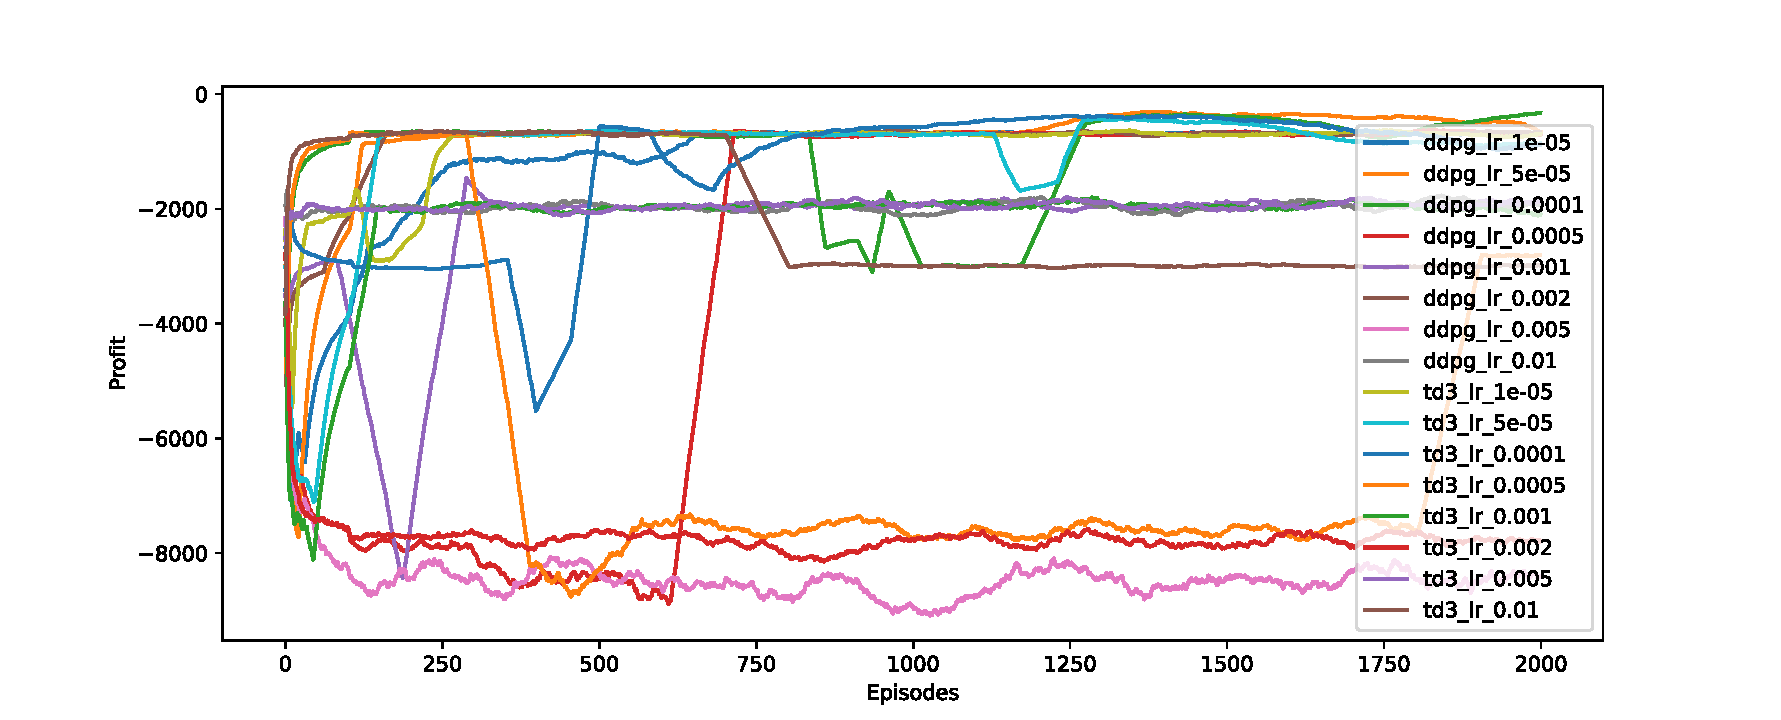
\includegraphics[width=\textwidth]{main/DDPG_learning_curve.pdf}
	\caption{Lernkurven von DDPG und TD3 mit unterschiedlichen Lernraten}
	\label{graphic:DDPGLearningCurve}
\end{figure}

Die Lernkurven der beiden sehr ähnlichen Verfahren DDPG und TD3 sind in Abbildung \ref{graphic:DDPGLearningCurve} dargestellt.
Für jeden der beiden Algorithmen wurden acht Trainingsläufe durchgeführt, die mit unterschiedlichen Lernraten parametrisiert wurden.
Der Standardwert liegt für beide Algorithmen bei $1e-3$.
Es wurden Trainingsläufe mit diesen Lernraten sowie kleineren und größeren durchgeführt.
Die beim Training beobachteten Muster gleichen sich sowohl bei den beiden Algorithmen als auch den unterschiedlichen Parametrisierungen.

Zu Beginn des Trainings ist bei einigen Läufen eine Verbesserung der gemittelten Returns, die primäre Leistungskennziffer, zu beobachten.
Allerdings kommt diese Verbesserung bei allen Algorithmen zum Erliegen und die Gewinnzone nie erreicht.

Betrachtet man die Zusammensetzung der Gewinne -- die Diagramme dazu befinden sich im Anhang -- erkennt man, dass ein Teil der Agenten durch das Setzen hoher Neupreise wenige Kunden mit hoher Rendite gewinnen konnte.
Die mit dem Neuverkauf erwirtschafteten Gewinne liegen jedoch nie über 100 in der Episode und damit deutlich niedriger als bei anderen Policies.
Ein Teil der Algorithmen verharrt auf Preisen, die niedriger sind als die Einkaufspreise.
Diese ziehen besonders viele Kunden an und erhöhen dadurch noch den Verlust.
Bei der Reduktion der Rückkaufkosten konnten einige Agenten akzeptable Leistungen erreichen, aber keiner der Algorithmen konnte mit dem Verkauf gebrauchter Produkte Geld einnehmen.
Einige der Agenten mussten sogar ständig dafür Strafe zahlen, dass sie keine Gebrauchtprodukte liefern konnten.

Die Trainingsdurchläufe zeigen, dass sich die Leistung oft ruckartig verändern.
Der dabei in den Lernkurven zu erkennende lineare Auf- oder Abstieg ist der Durchschnittsbildung über die letzten hundert Episoden geschuldet.
Tatsächlich findet die Änderung sprunghaft statt, wie man es an den Scatterplots ablesen kann.
Zahlreiche der Trainingsdurchläufe sind von starken Einbrüchen der Leistung geprägt.
Diese Instabilität bei DDPG und TD3 sind als Problem bekannt.

Die Tatsache, dass die Agenten lange auf einer Stelle bleibt und auch die gleichen verbesserungswürdigen Aktionen immer wieder ausführt, kann auf unzureichende Exploration schließen lassen.
Allerdings konnten auch eine verrauschte Aktionswahl zur besseren Exploration keine Verbesserung der Leistung erreichen.

\section{On-Policy-Learning -- A2C und PPO}
\label{section:main_ppo}
Die beiden On-Policy-Verfahren A2C und PPO gibt es für diskrete wie für stetige Aktionsräume.
Wegen der großen Zahl der Aktionen werden auch hier jedoch nur die stetige Variante trainiert.

\begin{figure}[htbp]
	\centering
	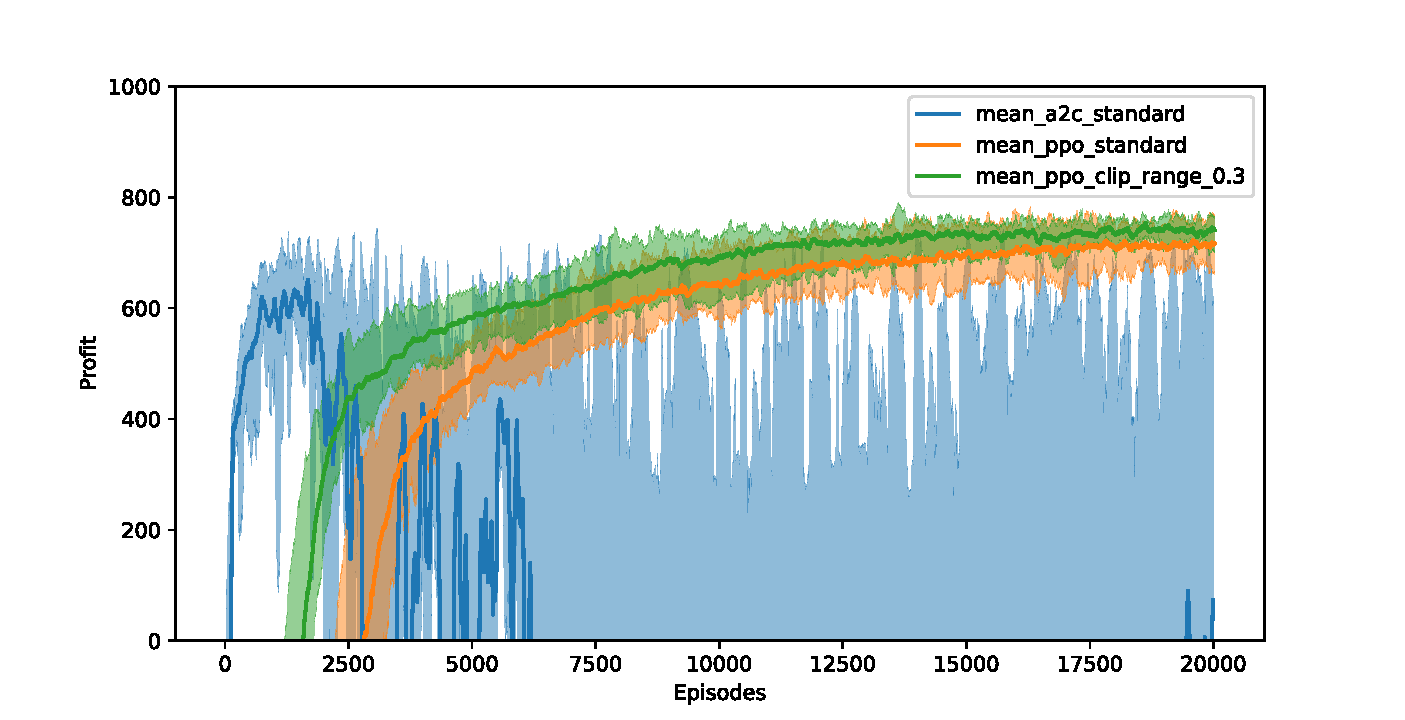
\includegraphics[width=\textwidth]{main/a2c_vs_ppo.pdf}
	\caption{Lernkurven von A2C und PPO auf dem Duopol mit unterbietendem Wettbewerber}
	\label{graphic:OnPolicyLearningCurves}
\end{figure}

Grafik \ref{graphic:OnPolicyLearningCurves} stellt die Lernkurven der Algorithmen dar.
Dabei wurde PPO mit zwei Hyperparametrisierungen verwendet, die sich im Parameter $\epsilon$ unterscheiden.
Das eine Mal wird $0.2$ wie im Originalpaper verwendet, das andere Mal $0.3$.
Jedes dieser Experimente wurde vier Mal unabhängig für eine Million Schritte (zweitausen Episoden) laufen gelassen.
Die Lernkurven verwenden wieder die laufenden Durchschnitte der Episodenreturns.
Der Bereich zwischen maximalem und minimalem Episodenreturns dieser vier Agenten ist eingefärbt.
Die Linie stellt ihren Durchschnitt dar.
In dieser Grafik wird der Verlustbereich ausgeblendet, um einen genaueren Vergleich im oberen Leistungsbereich zu ermöglichen.

Aus den Grafiken geht unmittelbar hervor, dass alle diese Agenten die Gewinnzone erreichen.
Sie erreichen alle Ergebnisse über 6000 pro Episode gute Ergebnisse.
Auf Grundlage dieser Ergebnisse kann man feststellen, dass die Parametrisierung mit $\varepsilon=0.3$ bessere Performance einbringt als die Standardparametrisierung, die wiederung A2C überlegen ist.
Allerdings liegt auch A2C in der Spitzenperformance nicht deutlich hinter den anderen Algorithmen.

Die Advantage-Actor-Critic-Agenten erreichen das hohe Leistungsniveau allerdings nach deutlich weniger Episoden als die PPO-Agenten.
Ihr Durchschnitt überschreitet die Schwelle zum Gewinn nach deutlich unter Episoden.
Allerdings ist das Training der A2C-Agenten ausgesprochen instabil.
\begin{figure}[htbp]
	\centering
	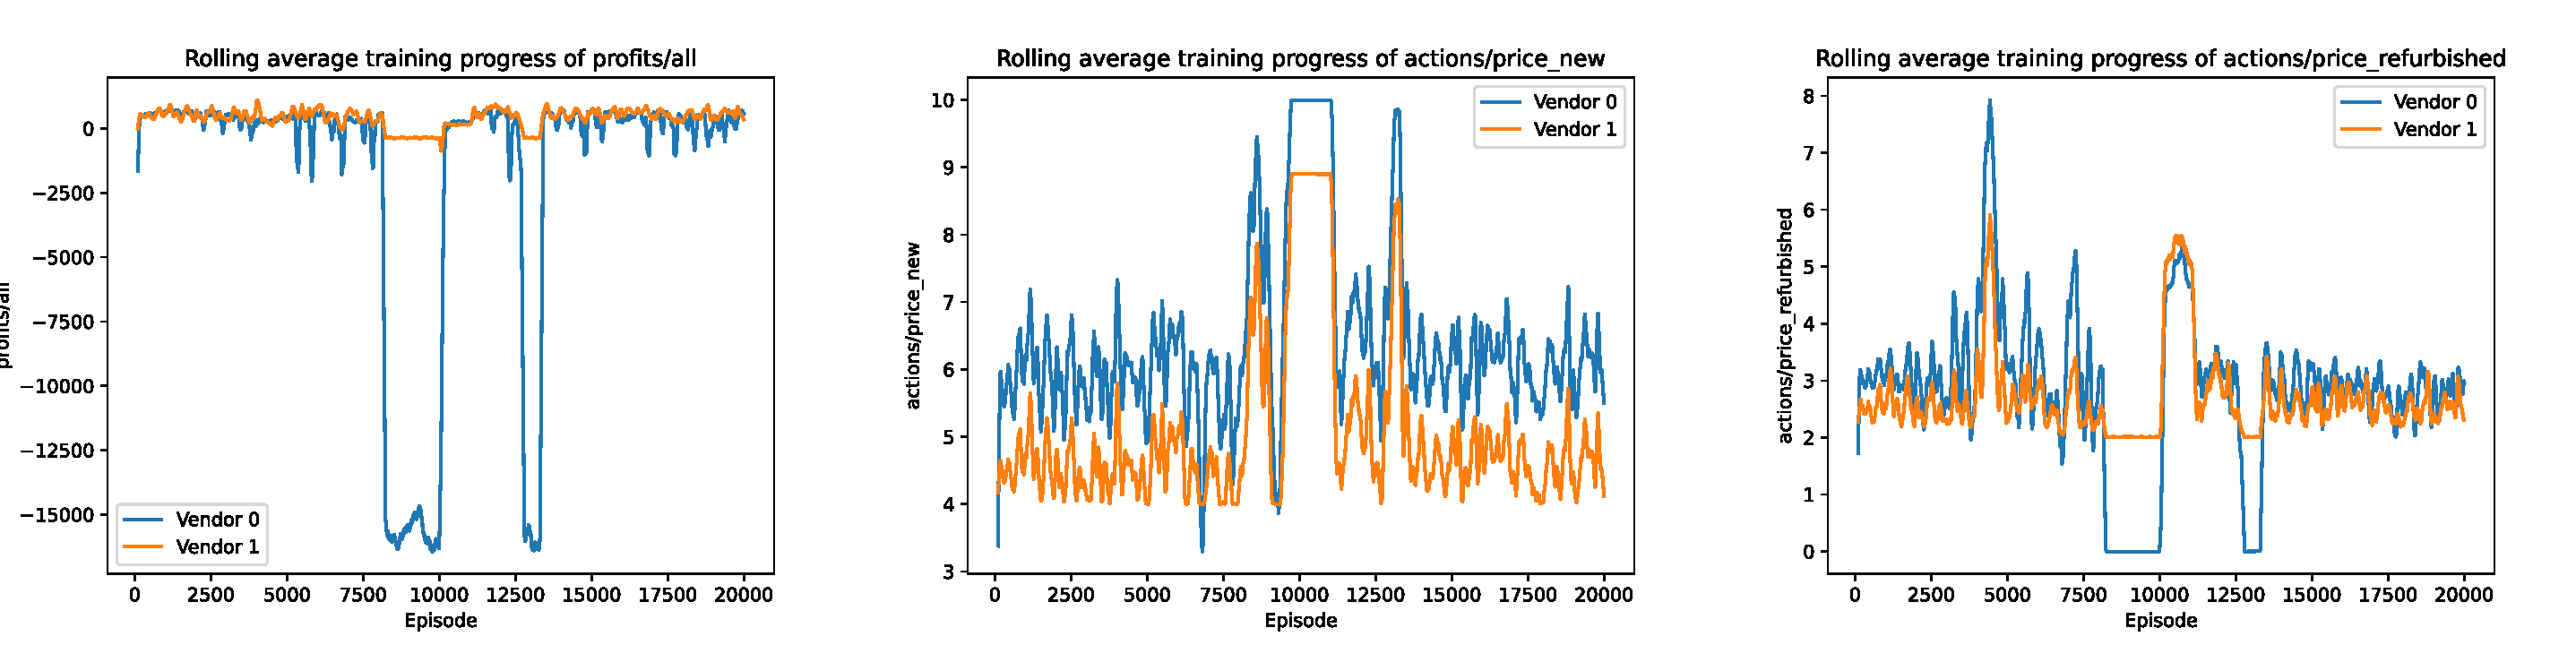
\includegraphics[width=\textwidth]{main/a2c_detailed_analysis.pdf}
	\caption{
		Detaillierte Betrachtung eines A2C-Trainingsdurchlaufes zur Visualisierung der Instabilität, wobei Vendor\_0 der RL-Agent und Vendor\_1 der regelbasierte, direkte Wettbewerber während des Trainings ist:
		(links) Lernkurve mit schnellem initialem Anstieg, danach Abstürze und Erholungen;
		(mitte) durchschnittliche Auswahl der Neupreise, zeigt erhebliche Schwankungen;
		(rechts) durchschnittliche Auswahl der Gebrauchtpreise, ebenfalls instabil
	}
	\label{graphic:A2CInstability}
\end{figure}
Die Grafik \ref{graphic:A2CInstability} stellt Details eines einzelnen A2C-Durchlaufes dar.
Es handelt sich dabei um einen typischen Durchlauf mit mittlerer Peak-Performance.
Man sieht, dass die Aktionsauswahl während des Trainings starken Schwankungen unterworfen ist.
Wie auch bei den anderen A2C-Agenten stürzt seine Leistung mitunter deutlich ab und fällt dabei weit in die Verlustzone.
Nicht immer erholen sich die Agenten davon, oft erhalten sie weiterhin schlechte Ergebnisse.
Diese heftigen Abstürze führen dazu, dass die Mittelwertlinie der A2C-Agenten in Abbildung \ref{graphic:OnPolicyLearningCurves} wieder unter 0 fällt, obwohl einige der Agenten weiterhin akzeptable Ergebnisse liefern.

Im Gegenzug dazu ist die Trainingsstabilität bei den PPO-Varianten deutlich höher.
Zwischen den vier Trainingsdurchläufen der PPO-Agenten gibt es nur geringe Unterschiede.
Die Leistungsentwicklung liegt in einem schmalen Band und Abstürze finden nicht statt.
Allerdings benötigt PPO in der Standardkonfiguration knapp 250 Episoden und in der Version mit $0.3$ als $\varepsilon$ ungefähr 160 Episoden, um die Gewinnzone zu erreichen.
Auch danach ist das Training langsam.
\begin{figure}[htbp]
	\centering
	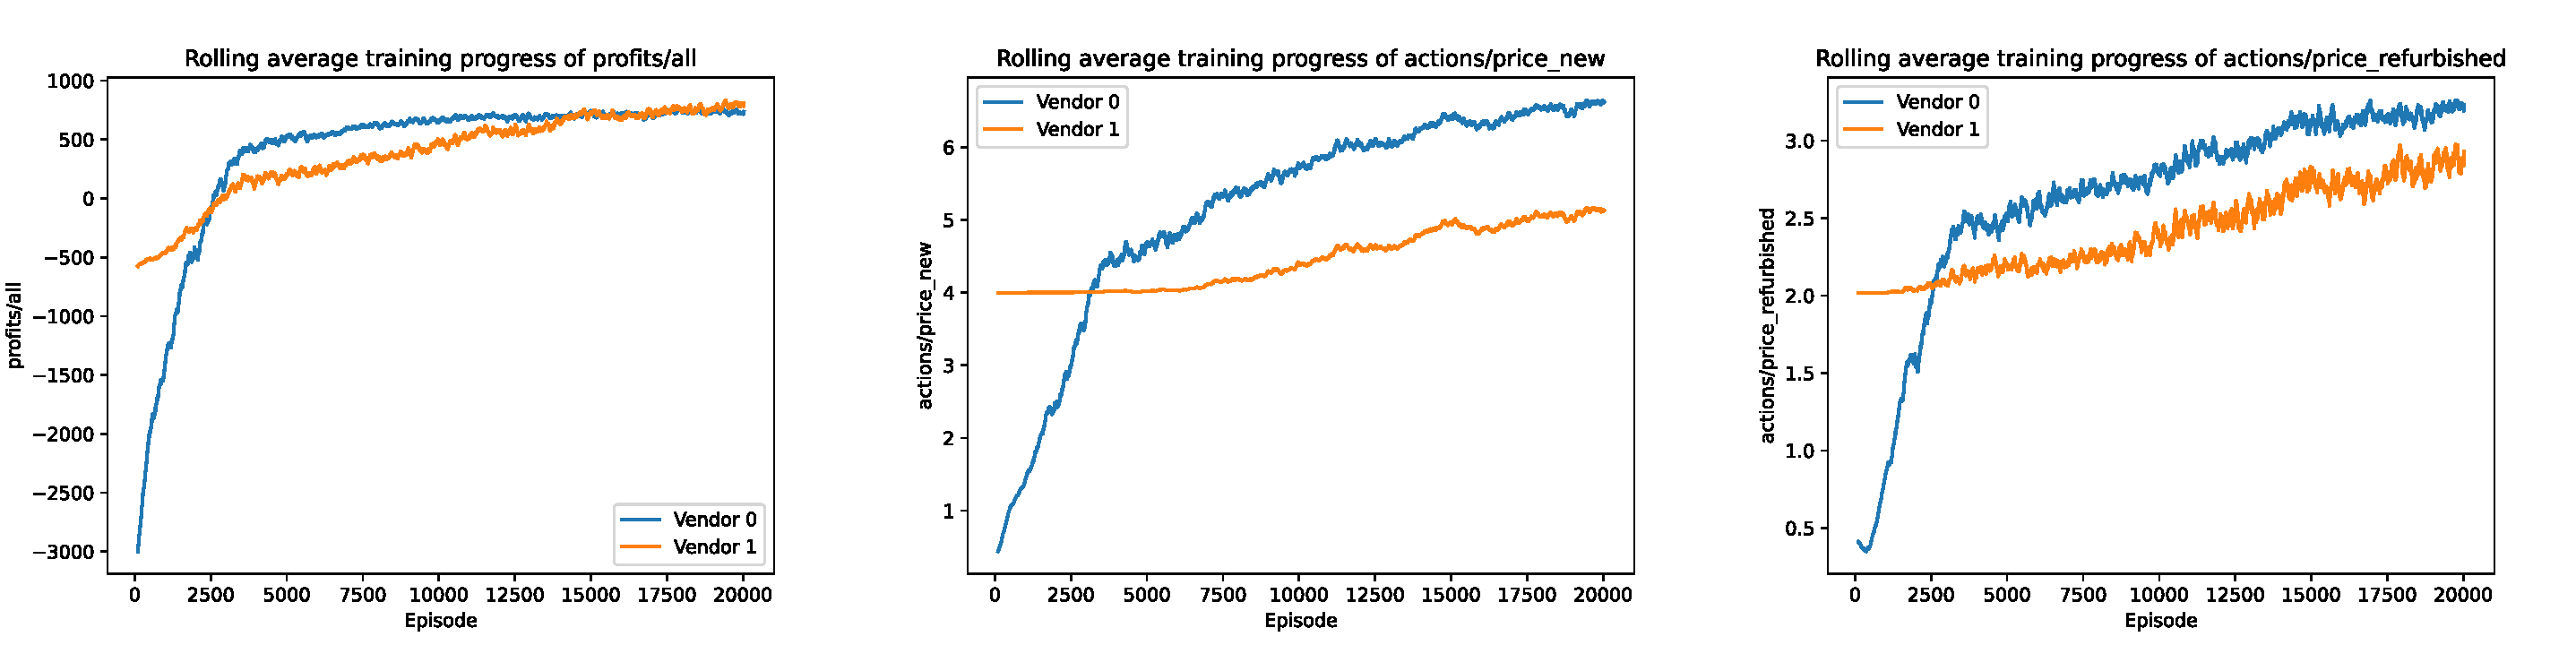
\includegraphics[width=\textwidth]{main/ppo_detailed_analysis.pdf}
	\caption{Detaillierte Betrachtung eines PPO-Trainingsdurchlaufes (Variante mit $\varepsilon=0.2$) analog zu Abbildung \ref{graphic:A2CInstability}}
	\label{graphic:PPOStability}
\end{figure}
In Abbildung \ref{graphic:PPOStability} ist ein detaillierter Blick in einen typischen PPO-Trainingsdurchlauf zu sehen.
Dessen durchschnittliche Performance steigt bis zum Ende auf über 8100, und weist bei Return und der Aktionsauswahl eine durchweg stabile Entwicklung auf.

Der Unterschied in der Lerngeschwindigkeit und -stabilität zwischen PPO zu A2C überrascht nicht, er existiert \textit{by design}.
Diese Experimente zeigen, dass PPO in seiner Intention, die Trainingsstabilität zu erhöhen, erfolgreich ist.
Diese Erhöhung der Trainingsstabilität findet dadurch statt, dass die Änderung der stochastischen Policy bei den Trainingsschritten begrenzt wird.
Aus dieser Begrenzung der Policyänderung ist die geringere Lerngeschwindigkeit dann eine logische Schlussfolgerung.

So lässt sich auch erklären, warum der Durchlauf mit $\varepsilon=0.3$ schneller trainiert.
Mit größerem $\varepsilon$ wird pro Sample eine größere Policyänderung erlaubt, was zu schnellerem Training führt.
Allerdings steigt damit wieder das Risiko von Instabilität, weshalb die Parametrisierung des PPO-Algorithmus einen Trade-off zwischen Trainingsgeschwindigkeit und Stabilität eröffnet.
Die Wahl des Standardparameters $0.2$ mag in diesen Experimenten konservativ erscheinen, $0.3$ ist ebenfalls noch recht stabil, weist aber bereits kleinere Abstürze auf.
Das Experiment [noch zu erstellen] im Anhang zeigt, wie sich PPO bei größerem $\varepsilon$ verhält.

Eine Beobachtung in Abbildung \ref{graphic:PPOStability} verdient noch einmal besondere Beachtung, weil sie zunächst paradox erscheint:
Obwohl der RL-Agent den regelbasierten Agenten nach etwas Training übertrifft, wird er später wieder wieder überholt.
Das erweckt den Eindruck, als ob der Agent im Verlaufe des Training schlechter würde.
Jedoch ist das Gegenteil der Fall.
Der PPO-Agent erlernt zunächst, die Preise für Neu- und Gebrauchtware höher zu setzen.
Dieses Training dauert aus inzwischen diskutierten Gründen relativ lange, aber bei Neuverkaufspreisen, die größer als vier sind, macht er die Erfahrung, dass der regelbasierte Wettbewerber ihn immer um 1 unterbietet.
Durch wechselseitiges Unterbieten führt eine Preisabwärtsspirale dazu, dass sich der Preis nur knapp überhalb des Einkaufspreises einpegelt.
Die dabei äußerst niedrige Rendite ermöglicht jedoch nur niedrige Gewinne, sodass der Agent in seinem weiteren Training die Erfahrung macht, dass er seinen Gewinn steigern kann, indem er seine Preise höher setzt.
Er wird dann zwar immer noch unterboten, allerdings nur um den Wert eins.
Dabei nimmt er in Kauf, dass mehr Kunden wegen des niedrigen Preises beim Konkurrenten kaufen und dieser auch an jedem Kunden noch mehr verdient.
Mit den Kunden, die der RL-Agent aber noch bekommt, kann er aber seine Gewinne im Vergleich zum niedrigpreisigen Markt dennoch steigern.
Der Effekt besteht also darin, dass der RL-Agent in Reaktion auf den ihn immer unterbietenden Konkurrenten diesem einen überproportionalen Gewinnanstieg erlaubt, um selbst mehr Gewinne machen zu können.
Dass sich dieser Effekt so wiederfindet, ist der Tatsache geschuldet, dass das einzige Optimierungskriterium für die Agenten der eigene Gewinn ist.
Eine Rewardformulierung, die ein Übertreffen des Konkurrenten mit einbezieht, wird in Abschnitt [wenn es noch im Scope ist] behandelt.

\section{Soft Actor Critic}
\label{section:main_sac}
Das in Abschnitt \ref{section:sac} erläuternte Soft-Actor-Critic-Verfahren ist in erster Linie für stetige Aktionsräume entwickelt worden und wird hier auch in der stetigen Variante genutzt.
Bei den hier gezeigten Ergebnissen wurde der Entropiekoeffizient $\alpha$ automatisch trainiert.
Er hat sich bei allen Trainingsdurchläufen bei etwa $1.5$ eingependelt.
Die Grafik ? im Anhang zeigt, dass unterschiedliche manuell eingestellte Entropiekoeffizienten ähnliche Trainingsergebnisse erreichen, wobei sich die Vermutung bestätigt, dass sehr niedrige Entropiekoeffizienten zu wenig Exploration bezwecken und Läufe mit deutlich höheren Entropiekoeffizienten bei schlechterer Leistung verharren.

\begin{figure}[htbp]
	\centering
	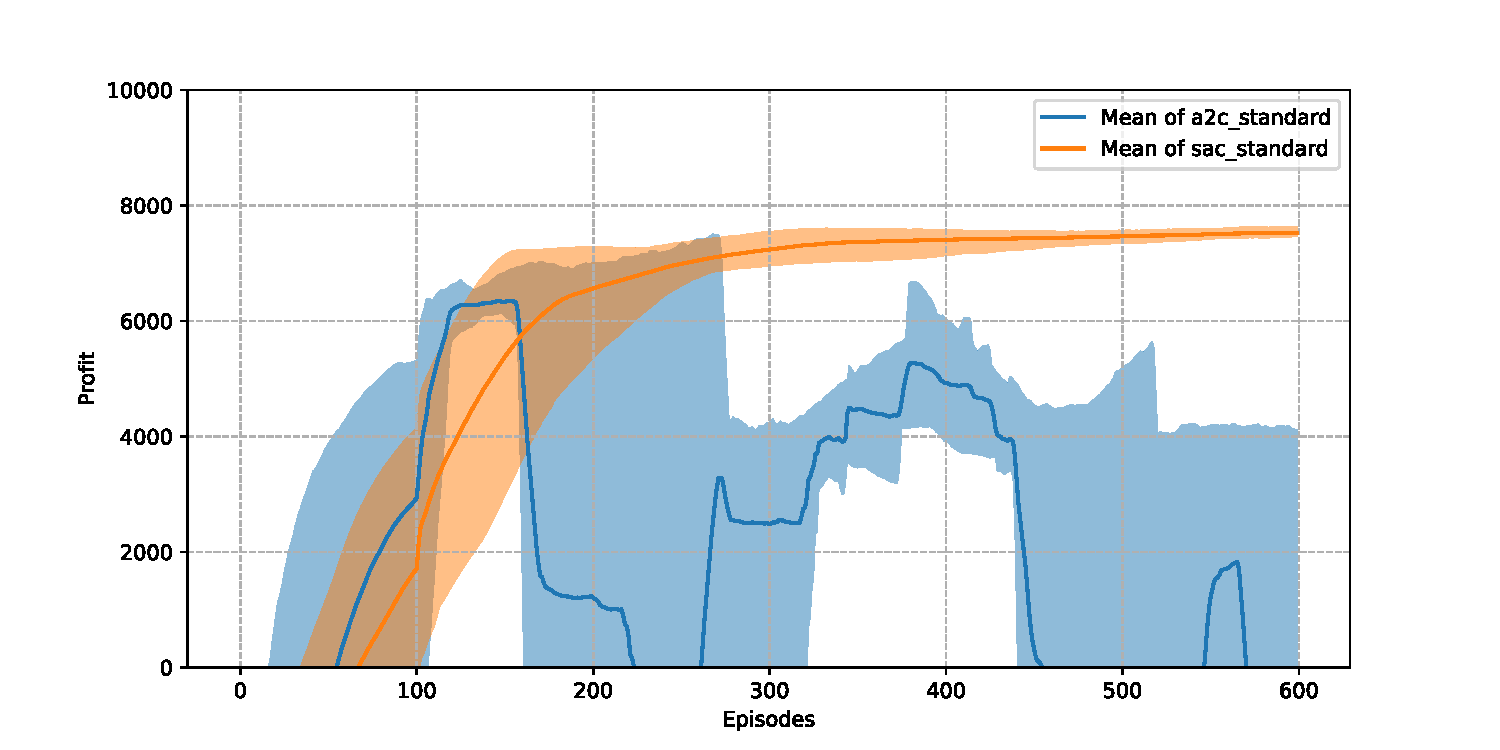
\includegraphics[width=\textwidth]{main/a2c_vs_sac.pdf}
	\caption{Lernkurve von Soft Actor Critic über 600 Episoden, A2C als Vergleich angegeben}
	\label{graphic:SACLearningCurve}
\end{figure}

Grafik \ref{graphic:SACLearningCurve} zeigt die Lernkurve von vier Soft-Actor-Critic-Agenten bei einem Trainingsdurchlauf mit 600 Episoden (300000 Schritte).
Zum Vergleich sind vier Trainingsdurchläufe mit A2C angegeben, die den aus Abschnitt \ref{section:main_ppo} bekannten Verlauf aufweisen.
Bei diesem Diagramm fällt ein sprunghafter Anstieg bei 100 Episoden auf.
Das liegt daran, dass ein laufender Durchschnitt verwendet wird, bei dem nach 100 Episoden die sehr schlechten Ergebnisse direkt am Anfang aus der Mittlung herausfallen.
Dieser Effekt tritt auch bei anderen dieser Lernkurven auf und hat keine weitere Bedeutung.

Soft-Actor-Critic wurde als Off-Policy-Algorithmus neben dem Erreichen von wettbewerbsfähigen Ergebnissen für zwei Hauptziele entwickelt:
Erstens soll es eine sehr hohe Sample Efficiency haben, was bedeutet, dass es beim Training deutlich weniger Schritten benötigt.
Zweitens soll SAC eine sehr hohe Trainingsstabilität haben.
Die Lernkurve bestätigt, dass Soft-Actor-Critic diese zwei Hauptziele erreicht.
Profitabel arbeitet der Agent nach etwa 70 Episoden, was nur leicht hinter A2C liegt und erheblich besser als PPO ist.
Spitzenperformance wird ähnlich wie bei A2C nach 250 bis 300 Episoden erreicht.
Der weitere Trainingsverlauf ist sehr stabil.
Alle vier Agenten bewegen sich für den Rest des Trainings in einem sehr schmalen Bereich, wobei der Durchschnittsreturn der Agenten bei etwa 7500 konstant bleibt.
Eine Verbesserung der Leistung findet nach etwa 350 Episoden nicht mehr statt.
Der Durchschnitt der acht SAC-Agenten liegt zwar dauerhaft über dem Durchschnitt der A2C-Agenten, aber gute A2C-Durchläufe erreichen durchaus ähnliche Spitzenperformance wie die SAC-Agenten.
Es ist ebenfalls festzustellen, dass die Leistung der SAC-Agenten signifikant hinter denen der PPO-Agenten bleiben, die zuverlässig über 8000 als Return erzielen.

\begin{figure}[htbp]
	\centering
	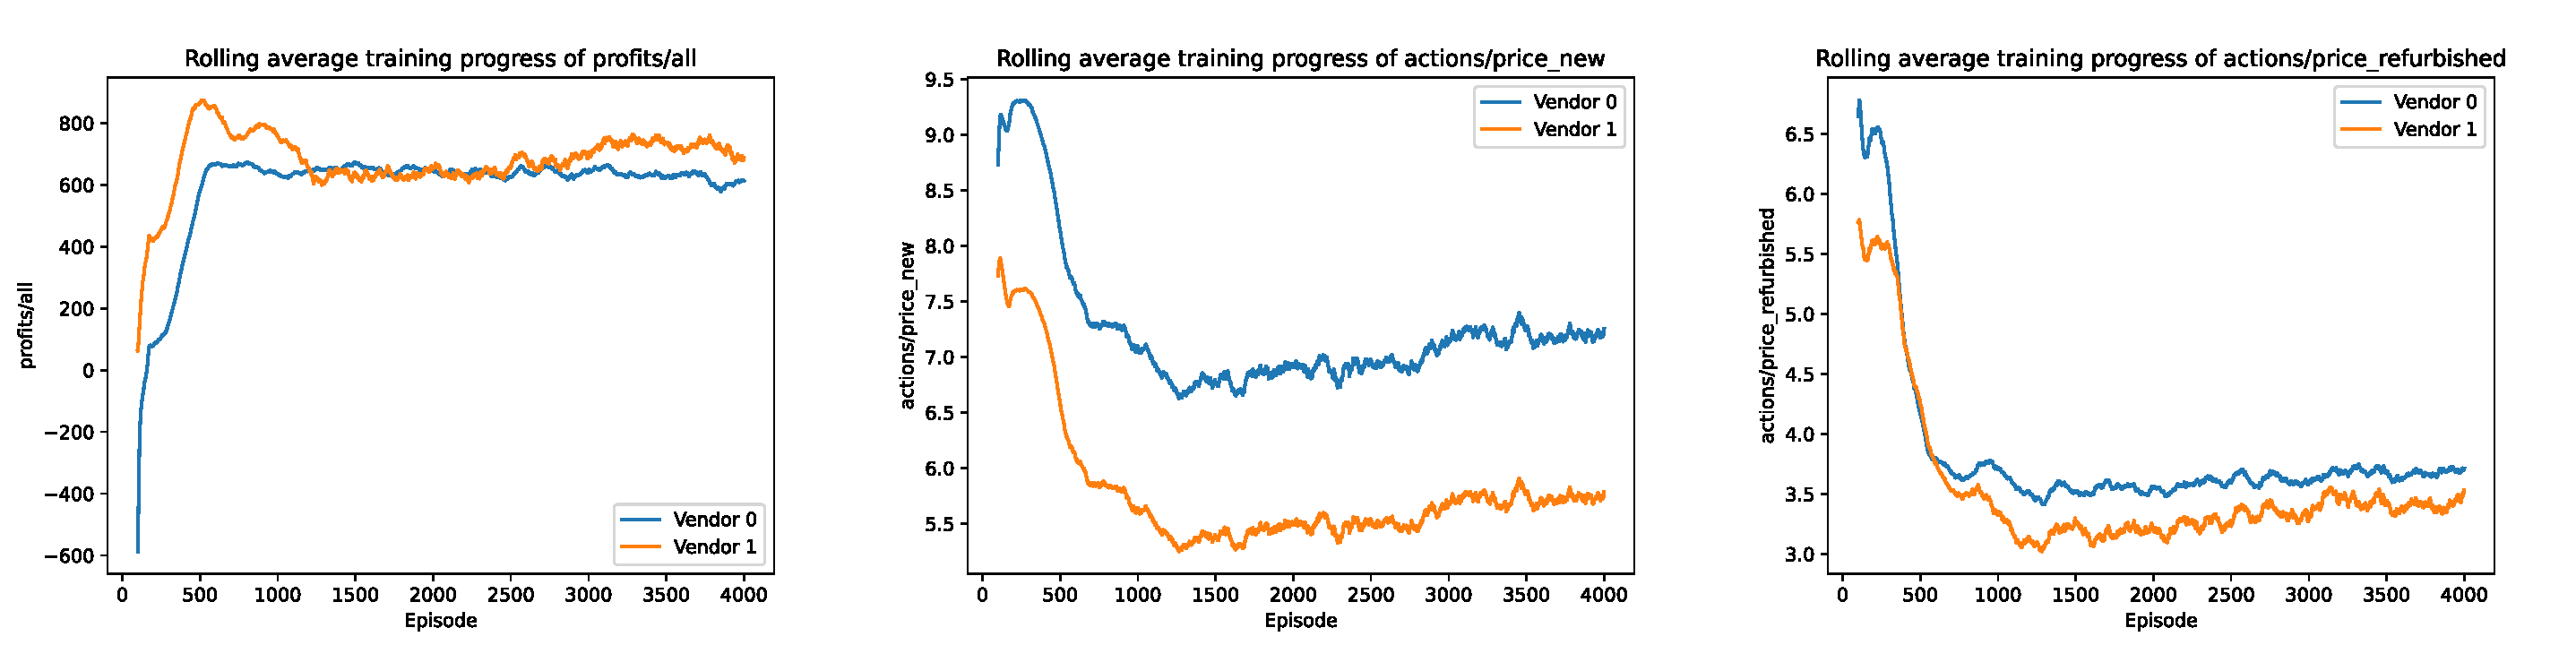
\includegraphics[width=\textwidth]{main/sac_detailed_analysis.pdf}
	\caption{Detaillierte Betrachtung eines SAC-Trainingsdurchlaufes}
	\label{graphic:SACDetails}
\end{figure}

Wie auch für die anderen Algorithmen wurde für SAC ein typischer Durchlauf und die gemittelten Aktionen in Abbildung \ref{graphic:SACDetails} abgedruckt.
Dieser ist stabil und weist abgesehen vom Start mit höheren Werten einen nicht unähnlichen Verlauf im Vergleich zum PPO-Durchlauf auf:
Zunächst sinken die Neupreise, steigen dann leicht an und enden bei 6,4 und 5,4, genau wie bei PPO.

Für die Frage >>Wie lange dauert das Training?<< gibt es zwei mögliche Kenngrößen.
Einmal kann die Anzahl der benötigten Samples bewertet werden, die Sample Efficiency, oder es kann die tatsächliche Zeit auf der Uhr harangezogen werden.
Letztere hängt stark von der Hardware sowie der Geschwindigkeit der Simulation im Vergleich zum Optimieren der Parameter ab.
Bei der für diese Experimente verwendeten Implementierung und Hardware benötigt das Training pro Schritt mit SAC etwa $3.7$ Mal so lang wie mit PPO.
Das Sammeln der Beispiele aus dem Markt nimmt bei PPO etwa 25\% der Trainingszeit ein, bei SAC nur etwa 6\%.
Die Geschwindigkeiten von A2C sind denen von PPO sehr ähnlich.
Rechnet man somit die tatsächliche Trainingszeit, relativiert sich der höhere Samplebedarf bei PPO.
Es wird allerdings klar, dass A2C in reinem Zeitbedarf den anderen Algorithmen deutlich überlegen ist.

\section{Den Konkurrenten übertreffen -- eine angepasste Rewardfunktion}
\label{section:mixed_reward_function}
In den bisher untersuchten Lernkurven erreichen die Agenten zwar sehr gute Profite, lassen sich aber vom regelbasierten Konkurrenten übertreffen.
In Abschnitt \ref{section:main_ppo} wurde bereits erklärt, dass dies nicht als Schwäche der Algorithmen zu deuten ist, sondern darauf auf die Rewardfunktion zurückgeführt werden kann, die nur eigenen Profit bewertet.
Nun ist die Maximierung des eigenen Profits keine ungeeignete Kenngröße, dennoch werden Unternehmen ungern ihren Konkurrenten in einem symmetrischen Markt mehr Gewinn überlassen als sich selbst.
Deshalb liegt es nahe, in der Belohnungsfunktion nicht nur die eigenen Profite zu bewerten, sondern auch, ob der Konkurrent übertroffen wird.

Eine Möglichkeit besteht darin, den Markt als \textit{Zero-Sum-Spiel} zu formulieren, indem die Belohnung genau die Differenz aus eigenem Gewinn und dem des Konkurrenten ist.
Diese Formulierung legt den klaren Fokus auf das Übertreffen des Konkurrenten und eröffnet weiterhin möglicherweise das Marktszenario für Erkenntnisse aus der Spieltheorie für Zero-Sum-Spiele.
Allerdings diese Formulierung nicht praxistauglich, weil das Ziel der Profitmaximierung gar nicht bewertet wird.
So kann es passieren, dass bei einer Optimierung auf Differenz zwar der Konkurrent deutlich übertroffen wird, allerdings bei insgesamt niedrigen Gewinnen.

Deshalb wurde für die folgende Versuchsreihe eine gemischte Rewardfunktion verwendet.
Sie berechnet einfach die Summe aus Profit und Differenz zum Konkurrenten.
Für diese Experimente wurden beide Summanden gleich gewichtet, es könnte aber noch ein Hyperparameter eingefügt werden, um die beiden Ziele Profitmaximierung und Übertreffen des Konkurrenten zu balancieren.

\begin{figure}[htbp]
	\centering
	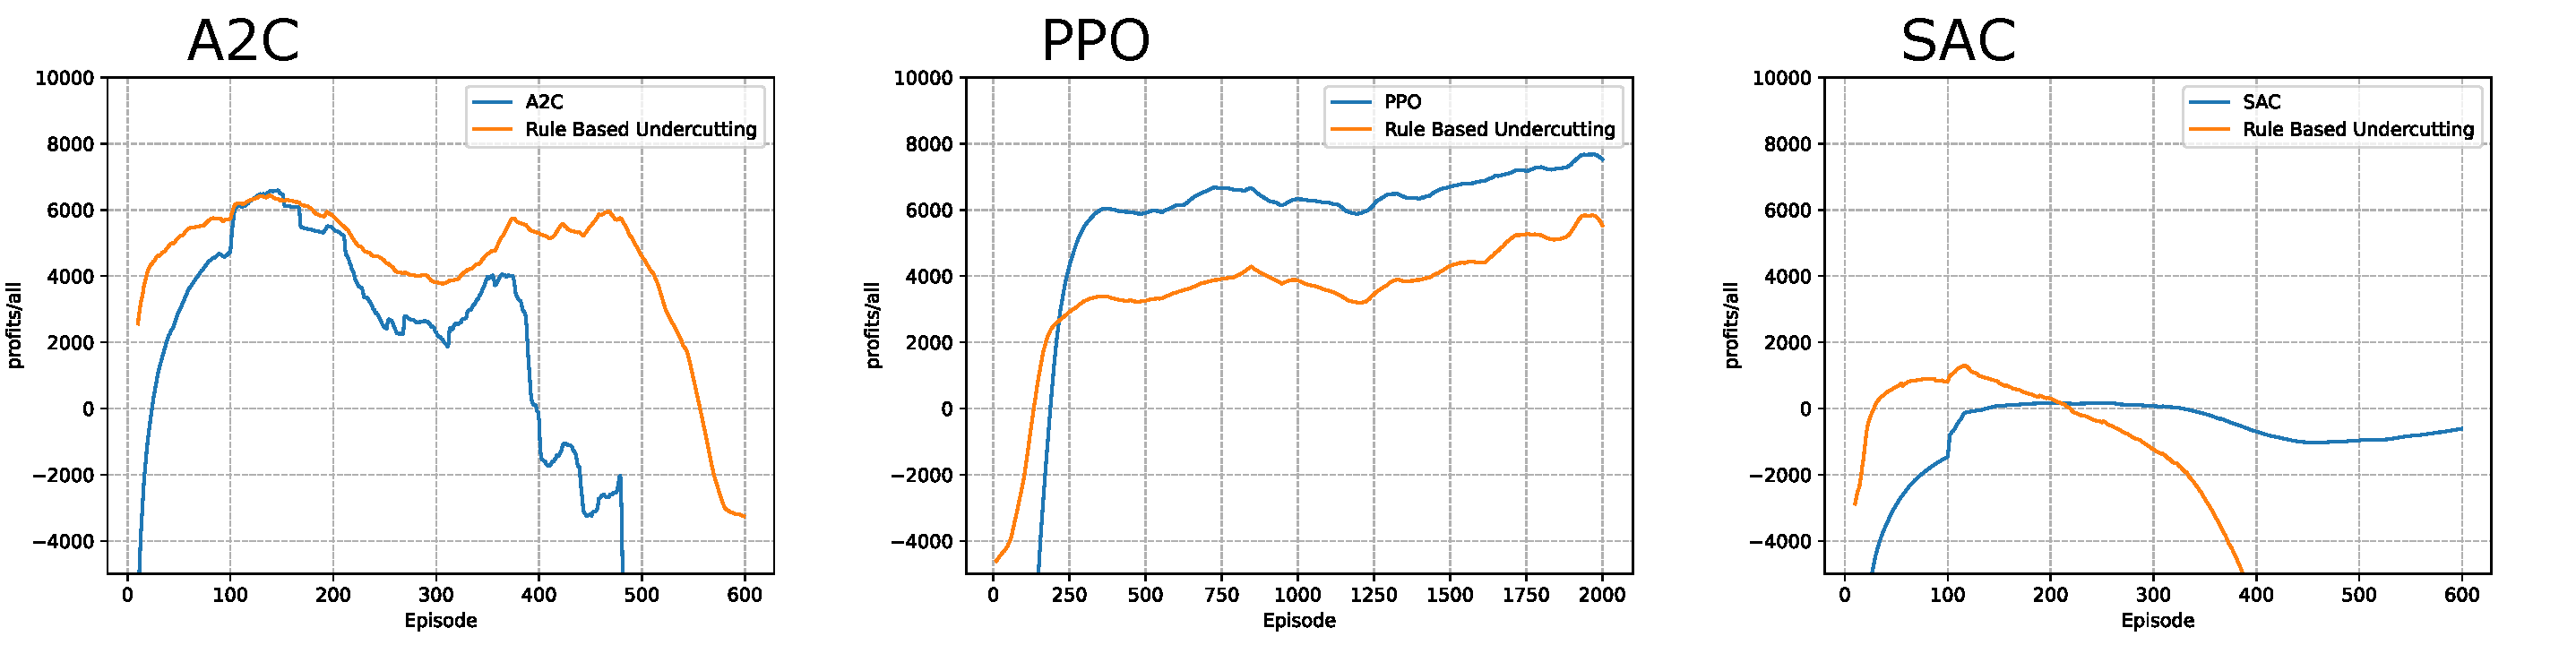
\includegraphics[width=\textwidth]{main/lineplot_mixed_rewards.pdf}
	\caption{Repräsentative Durchläufe der Algorithmen bei gemischter Rewardfunktion}
	\label{graphic:LineplotMixedRewards}
\end{figure}

Im Anhang sind die Lernkurven der Algorithmen mit gemischter Rewardfunktion im vergleich zur Standardrewardfunktion abgedruckt (Abbildungen \ref{graphic:MixedRewardsA2C}, \ref{graphic:MixedRewardsPPO} und \ref{graphic:MixedRewardsSAC}).
Wie erwartet liegen die Gewinne der Agenten niedriger als bei der anderen Rewardfunktion (schließlich sind Gewinne nicht mehr das alleinige Optimierungskriterium), allerdings fällt dieser Unterschied bei den Algorithmen unterschiedlich aus.
Insbesondere erhöht sich durch den Wechsel der Rewardfunktion die Instabilität bei allen Algorithmen.
Ob das Ziel, neben guten Gewinnen die Konkurrenz zu überholen, erreicht wird, zeigt Abbildung \ref{graphic:LineplotMixedRewards}.
Obwohl der A2C-Durchlauf wieder Probleme mit Instabilität zeigt, erreicht er ein durchschnittliches Maximum von 7900, der Konkurrent nur 7200.
Er überholt also bei der veränderten Rewardfunktion den regelbasierten Konkurrenten, und erhält gleichzeitig gute Gewinne.
Beim PPO-Durchlauf ist genau das zu sehen, was Ziel der Anpassung der Rewardfunktion war:
Der PPO-Agent bleibt nach dem ersten Übertreffen des Konkurrenten diesem über das gesamte Training hinweg voraus und erreicht ein Maximum von 8000 im Vergleich zu 6100 des regelbasierten Konkurrenten.
Der Soft-Actor-Critic-Durchlauf erreicht nach der gemischten Rewardfunktion sogar die besten Ergebnisse, obwohl der Agent selbst in die Verlustzone rutscht.
Er hat eine Policy gefunden, bei der der regelbasierte Konkurrent ständig Strafen zahlen muss, weil er keine gebrauchten Produkte liefern kann.
Die Details zu diesem Durchlauf sind interessant und in Abbildung \ref{graphic:ExplanationUnnormalSAC} im Anhang erläutert.
Aus Sicht der Algorithmenanalyse ist es ein bemerkenswertes Resultat, dass der SAC-Agent dazu fähig war, eine solche Strategie zu explorieren und zu entwickeln.
Für die praktische Verwendung ist diese Policy allerdings nicht geeignet.
Der Profit des Agenten sollte bei der Wahl der Rewardfunktion höher gewichtet werden.

\section{Training gegen die eigene Policy}
Die in den Abschnitten \ref{section:main_ddpg}, \ref{section:main_ppo} und \ref{section:main_sac} betrachteten Durchläufe trainierten die RL-Agenten alle gegen den in Abschnitt \ref{section:rulebased} definierten regelbasierten Wettbewerber.
Das erfüllt die theoretischen Anforderungen eines Markov-Entscheidungsprozesses, stellt jedoch für praktische Anwendungen eine Reihe von Problemen auf.
Erstens muss dafür die Policy des Konkurrenten bekannt sein.
Weil jedoch davon ausgegangen werden kann, dass der Konkurrent seine Preisstrategie nicht verraten wird, müsste sie unter Inkaufnahme von Ungenauigkeiten aus historischen Daten geschätzt werden.
Zweitens ist die mittels RL trainierte Strategie nur gegen diese bestimmte regelbasierte Strategie gerichtet.
Ändert der Wettbewerber seine Preisstrategie plötzlich, schwächt das die Performance der RL-Strategie und macht neues Training erforderlich.
Um jedoch die neue Strategie für das erneute RL-Training verstehen zu können, werden wieder historische Daten benötigt, die zunächst nicht vorliegen.

Deshalb wünscht man sich eine Strategie, die gegen möglichst viele Wettbewerberstrategien bestehen kann, nicht auf eine spezielle overfittet ist.
Deepmind hatte eine ähnliche Herausforderung beim Training von Go- und Schachstrategien, das sie durch Self-Play gelöst haben. \cite{Silver2017, https://doi.org/10.48550/arxiv.1712.01815}
Für diesen Markt wurde eine Self-Play Variante entwickelt, bei der ein RL-Agent weiterhin auf einem Duopol-Markt trainiert, aber die Policy des Wettbewerbers die eigene Policy ist.
In der programmiertechnischen Umsetzung wird dann für den Gegner ein Zeiger auf den RL-Agenten übergeben, der schließlich auch die Policyfunktion implementiert.
Dadurch, dass der Agent stets gegen sich selbst spielt, wird die Markov-Eigenschaft verletzt, dennoch zeigen die Ergebnisse Trainingserfolg.
Die Motivation hinter Self-Play ist, dass der Agent einerseits stets einem ebenbürtigen Gegner gegenübersteht, aber andererseits auch, dass er ständig Strategien gegen die eigene entwickelt, die dann wiederum herausgefordert werden.
Dadurch soll der Agent gegen eine Vielzahl von Policies gestählert werden.
Experimente mit Self-Play wurden mit den Algorithmen durchgeführt, die sich in der vorangegangenen Analyse als grundsätzlich geeignet für diesen Markt erwiesen haben: A2C, PPO und SAC.
Dabei wurde die gesamte Versuchsreihe mit der normalen Rewardfunktion und der gemischten Rewardfunktion aus Abschnitt \ref{section:mixed_reward_function} durchgeführt.

\begin{figure}[htbp]
	\centering
	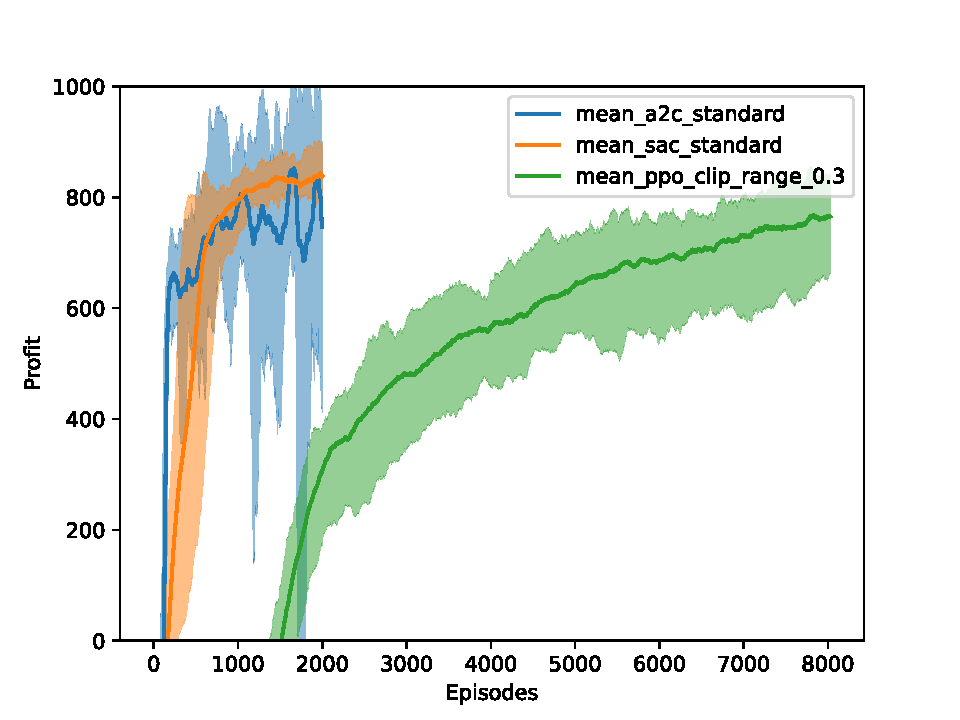
\includegraphics[width=\textwidth]{main/self_play.pdf}
	\caption{Lernkurve von A2C, PPO und SAC beim Self-Play; die Algorithmen wurden über 2000 Episoden trainiert}
	\label{graphic:SelfPlayLearningCurve}
\end{figure}
In der Abbildung \ref{graphic:SelfPlayLearningCurve} sind die Lernkurven der drei Algorithmen beim Training gegen sich selbst abgedruckt.
Die Lernkurven bei gemischter Rewardfunktion sehen ähnlich aus und sind im Anhang in Abbildung \ref{graphic:SelfPlayMixedLearningCurve} abgedruckt.
Diese Kurven zeigen zunächst, dass Lernerfolg bei allen dieser drei Agenten erreicht wird.
Sie sind aber alleine nicht aussagekräftig, ob die Agenten sich tatsächlich gegen die Konkurrenz behaupten können.
Deshalb dürfen auch die Returns dieser Lernkurven nicht mit den aus den vorigen Abschnitten verglichen werden.

\begin{figure}[htbp]
	\centering
	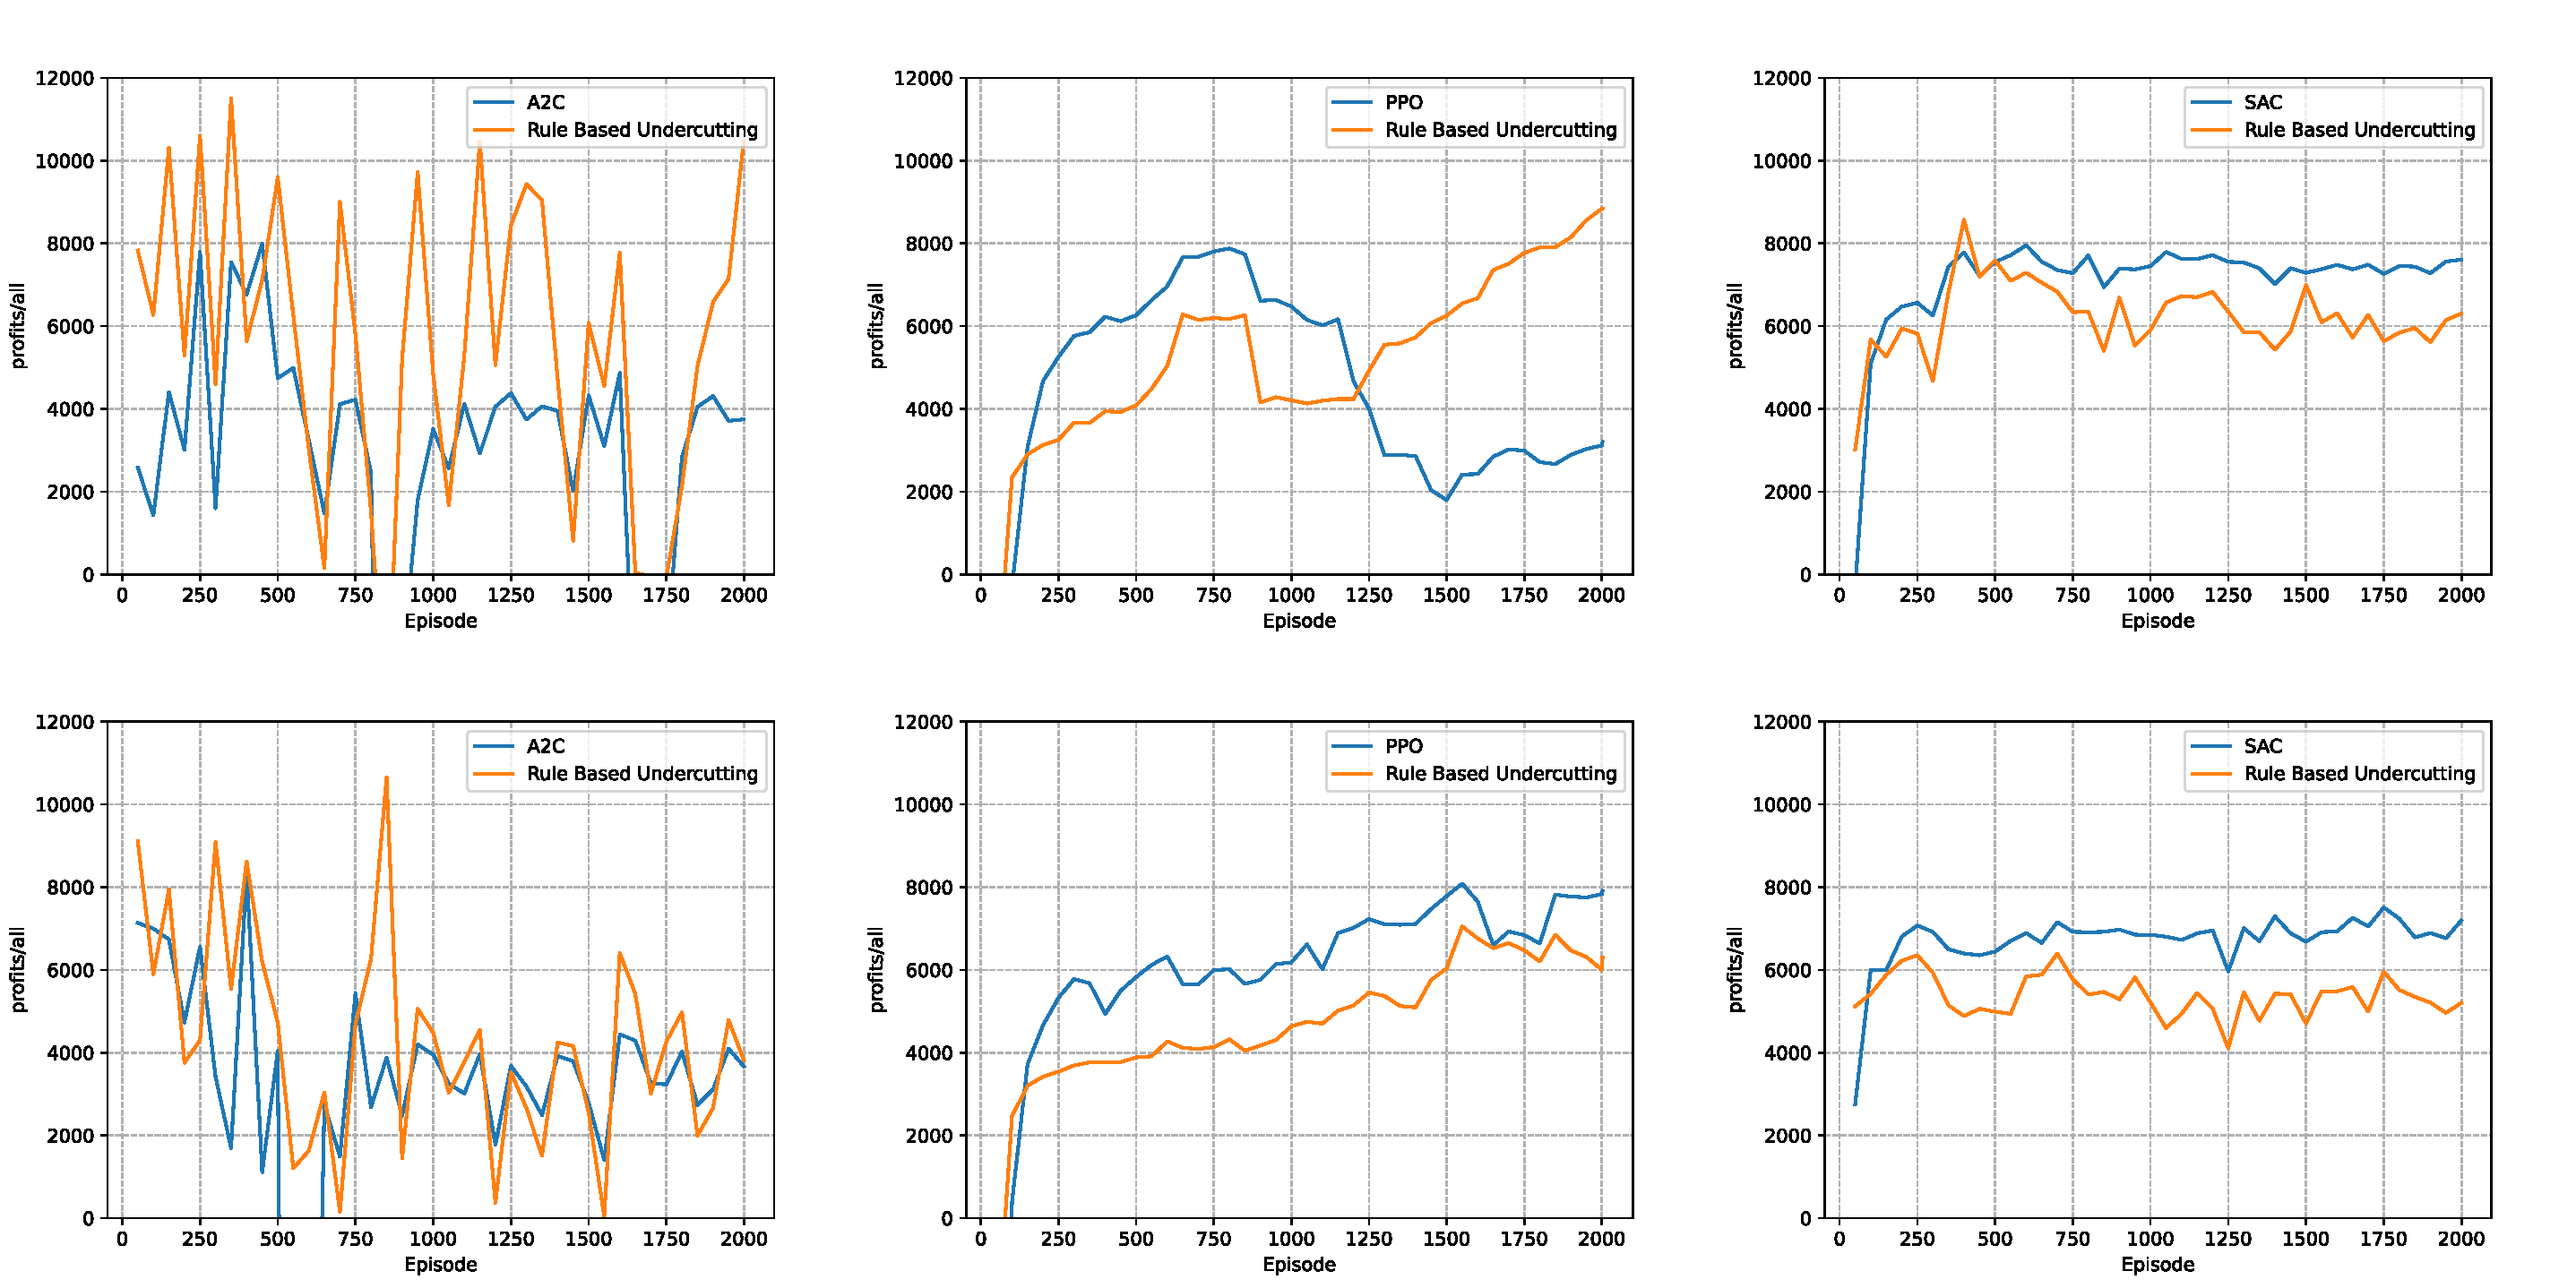
\includegraphics[width=\textwidth]{main/self_play_detailed.pdf}
	\caption{Repräsentative Self-Play Durchläufe; Spaltenweise nach Agenten: (links) A2c, (mittig) PPO, (rechts) SAC; obere Zeile mit normaler Rewardfunktion, untere Zeile mit gemischter Rewardfunktion}
	\label{graphic:SelfPlayDetails}
\end{figure}
Um Vergleichbarkeit herstellen zu können, wurde während des Self-Plays alle 50 Episoden ein Modell gespeichert und jedes dieser Modelle anschließend für 25 Episoden getestet.
Damit wurden akurate Lernkurven erstellt, die das beim Self-Play trainierte Modell mit dem regelbasierten Agenten vergleichen.
Für die drei Algorithmen und die zwei Rewardfunktionen wurde ein mittlerer Durchlauf ausgewählt und in der Abbildung \ref{graphic:SelfPlayDetails} veranschaulicht.
Bei beiden Rewardfunktionen haben die Agenten den Markt erfolgreich erlernt und können sich auch in dem Benchmark gegen den regelbasierten Konkurrenten behaupten.
So liegen die Spitzenwerte aller Agenten im Benchmark bei 8000 oder knapp darunter, allerdings mit starken Schwankungen bei A2C.
Von den A2C-Agenten erreichten einige kein Niveau von 5000.
Die Auswirkungen der gemischten Rewardfunktion sind gerade bei A2C und SAC deutlich.
Dass während des Trainings die Differenz zwischen eigenem und gegnerischen Profit mit als Optimierungskriterium verfolgt wird, führt tatsächlich dazu, dass der durch Self-Play trainierte Agent den regelbasierten Wettbewerber nicht vorbeiziehen lässt (A2C) oder ihn stärker abhängt (SAC).
Obwohl die Benchmarkergebnisse erwartungsgemäß nicht ganz an die Ergebnisse des Trainings direkt gegen den regelbasierten Agenten heranreichen, so sind sie nahe daran.
Das ist bemerkenswert, da diese Erfolge erreicht wurden, ohne den regelbasierten Wettbewerber je vorher gesehen zu haben.
Damit können diese Ergebnisse als erfolgreich gewertet werden und die Fähigkeiten vom Training gegen die eigene Policy in diesem Experiment bestätigt werden.

\section{Partielle Beobachtungen}
Für die Markov-Eigenschaft ist ein sechsdimensionaler Aktionsraum erforderlich.
Jedoch ist die Beobachtung mancher der verwendeten Größen in der Praxis nicht machbar.
So wird der Konkurrent sich nicht ins Lager schauen lassen, und die Anzahl der Produkte in Zirkulation ist schwer zu schätzen.
Deshalb drängt sich die Frage auf, ob die Algorithmen auch ohne diese beiden Informationen funktionieren.

\begin{figure}[htbp]
	\centering
	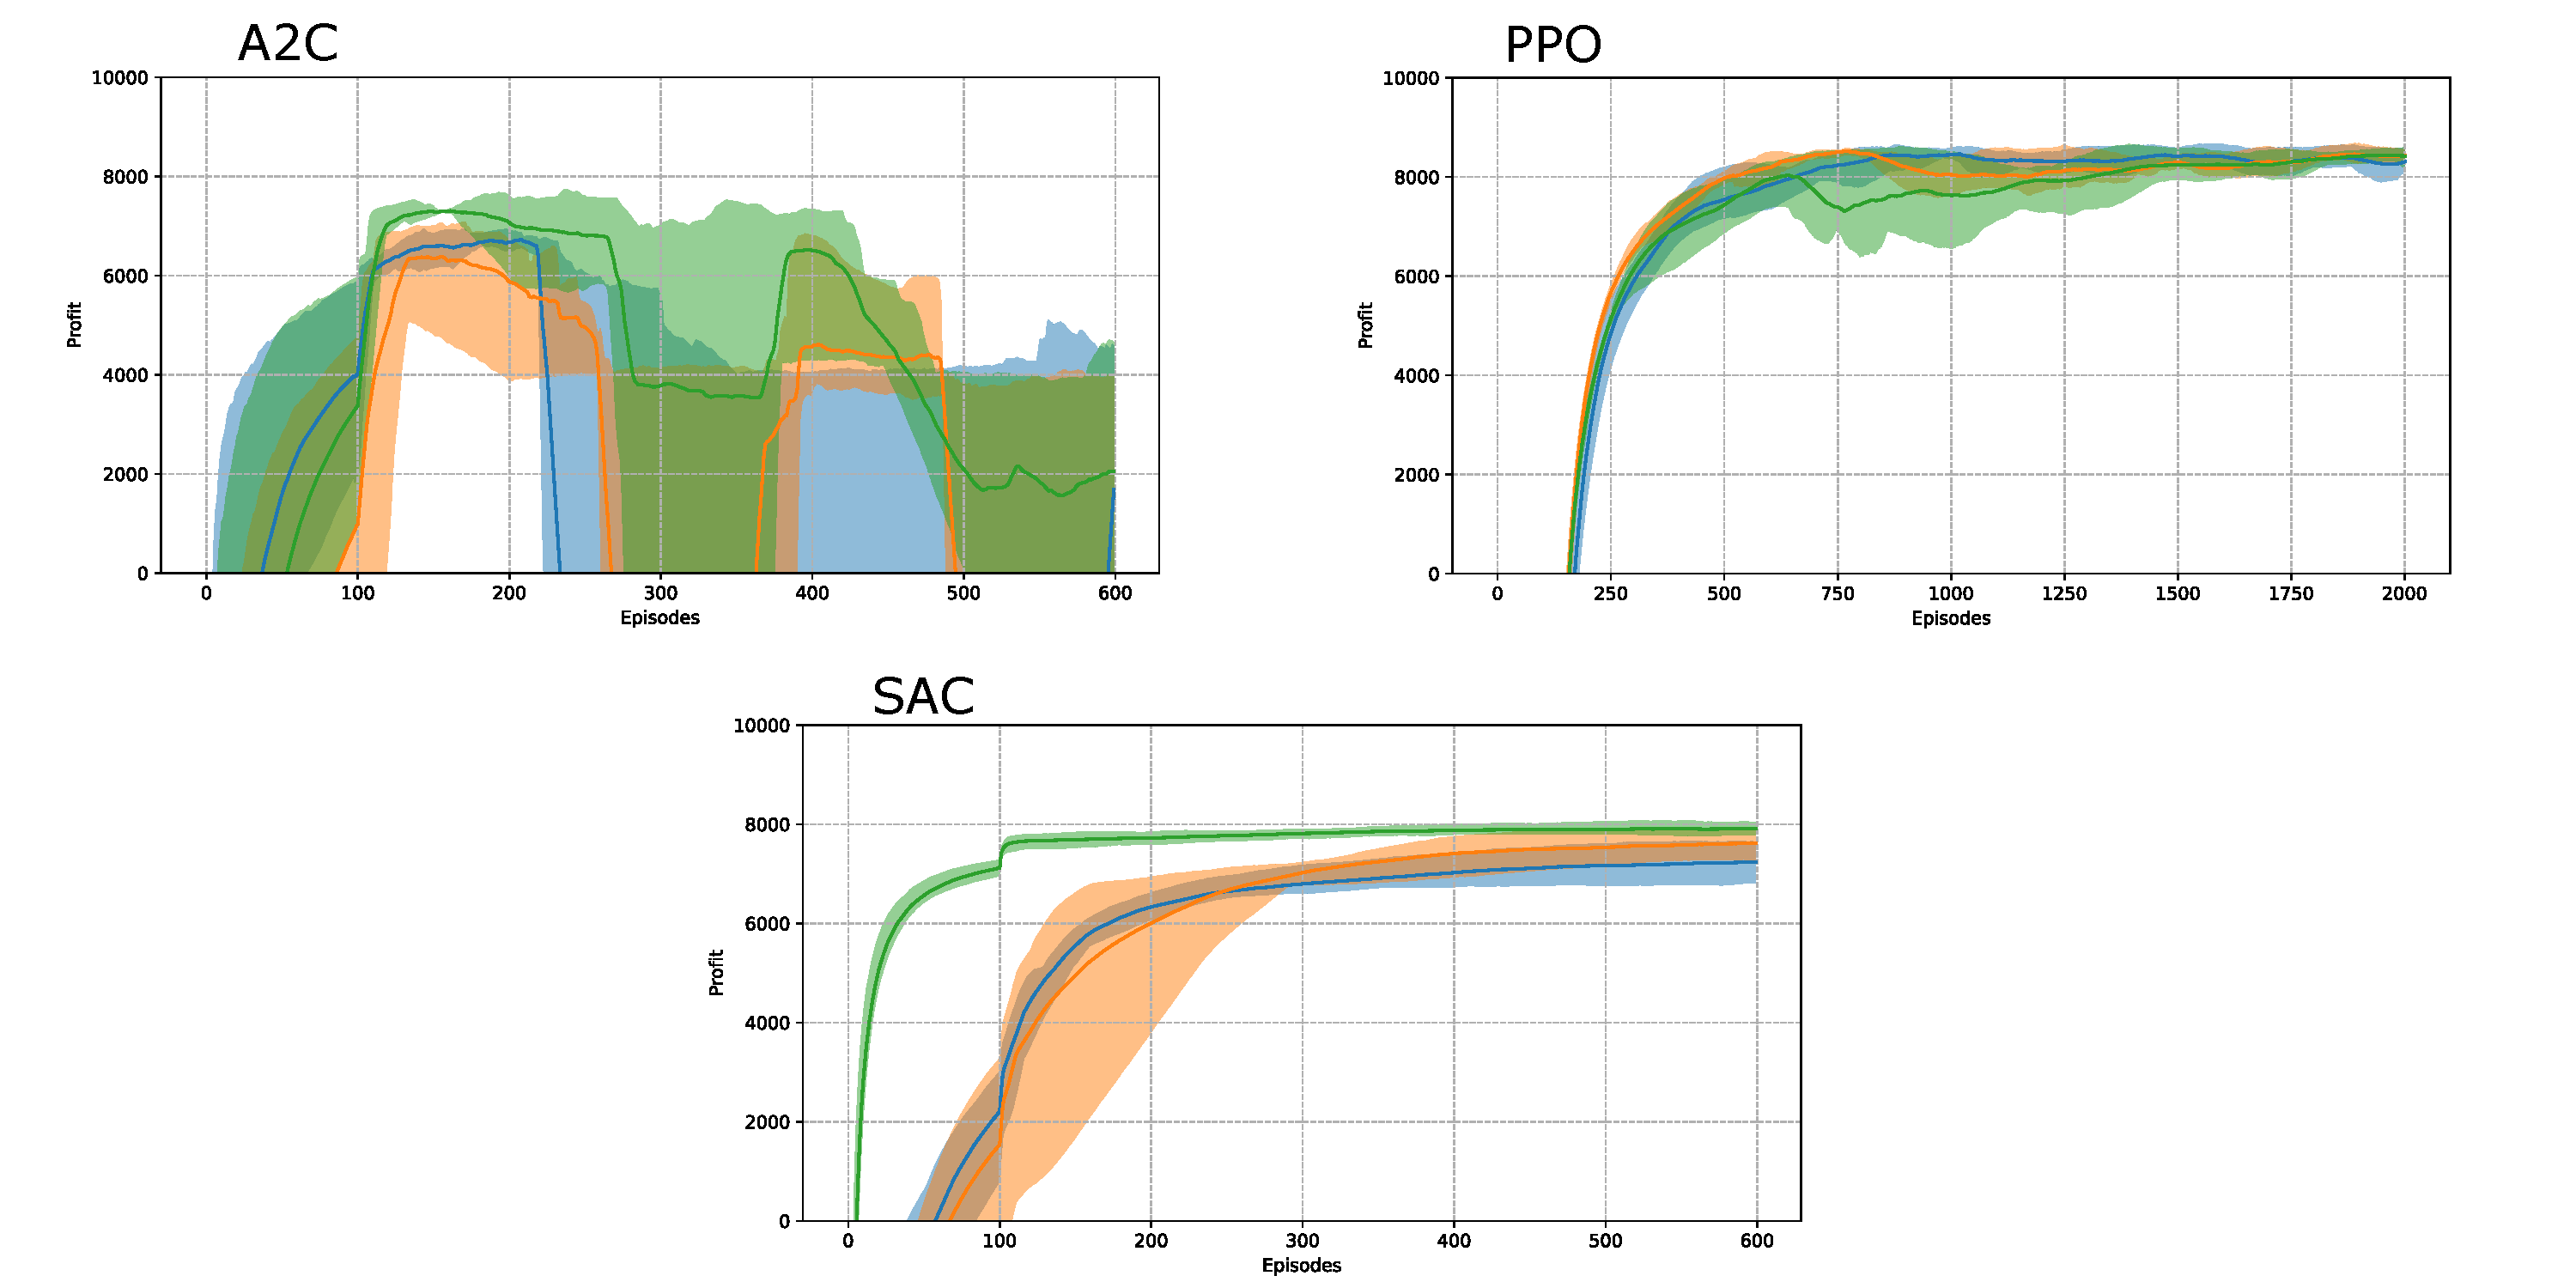
\includegraphics[width=\textwidth]{main/partial_observation.pdf}
	\caption{Lernkurven von A2C, PPO und SAC bei vollständiger im Vergleich zu partieller Beobachtung; (blau) vollständige Beobachtung, (orange) Lagerstand des Konkurrenten wird nicht bereitgestellt, (grün) Lagerstand des Konkurrenten und Anzahl der Produkte in Zirkulation werden nicht bereitgestellt}
	\label{graphic:PartialObservation}
\end{figure}

In Abbildung \ref{graphic:PartialObservation} sind die Lernkurven der drei Algorithmen beim Training gegen die unterbietende, regelbasierte Strategie dargestellt.
Das Ergebnis fällt dabei äußerst überraschend aus.
Die Erwartung, dass weniger Informationen zu schlechteren Ergebnissen führen müssten, erfüllt sich nicht.
Bis auf eine leicht verschlechterte Stabilität ist die Performance bei PPO ähnlich.
Die leicht schlechtere Stabilität ist durch des Fehlens von Informationen leicht erklärt.
Bei A2C verbessert sich ohne diese Informationen die Performance, und SAC sogar deutlich.
Während der SAC-Agent, dem nur der Lagerstand des Konkurrenten vorenthalten wird, recht ähnliche, leicht verbesserte Ergebnisse wie der mit vollständiger Information erzielt, ist der, bei bei denen zusätzlich die Information über die Anzahl der Produkte in Zirkulation fehlt, deutlich besser.
Es senkt sich nicht nur die Zeit bis zum Erreichen der Spitzenperformance auf unter 100 Episoden, sondern es verbessert sich sogar die endgültige Performance.
Damit reicht die Leistung näher, aber nicht ganz an die von PPO heran.
Das ist eine wichtige Erkenntnis mit Blick auf die praktische Anwendbarkeit, und dennoch stellt sich die Frage, wie sich die unerwartet gute Leistung mit unvollständiger Information erklären lässt.

Zur Erklärung ist zunächst heranzuführen, dass die ausgelassenen Informationen nur eine nachgeordnete Rolle spielen.
Sie erklären zwar zu einem Teil den künftigen Zug des Konkurrenten und die Anzahl der verkaufswilligen Eigentümer, allerdings sind die Auswirkungen so indirekt, dass sie schwer für die Verbesserung einer Policy zu verwerten sind. \footnote{Die regelbasierten Konkurrenten verwenden diese Information auch nicht}
Ein höherdimensionaler Beobachtungsraum stellt zudem grundsätzlich für die Agenten eine Herausforderung dar.
Es steigt dann der Bedarf an Samples, Muster in den Daten sind schwerer zu erkennen.

\begin{figure}[htbp]
	\centering
	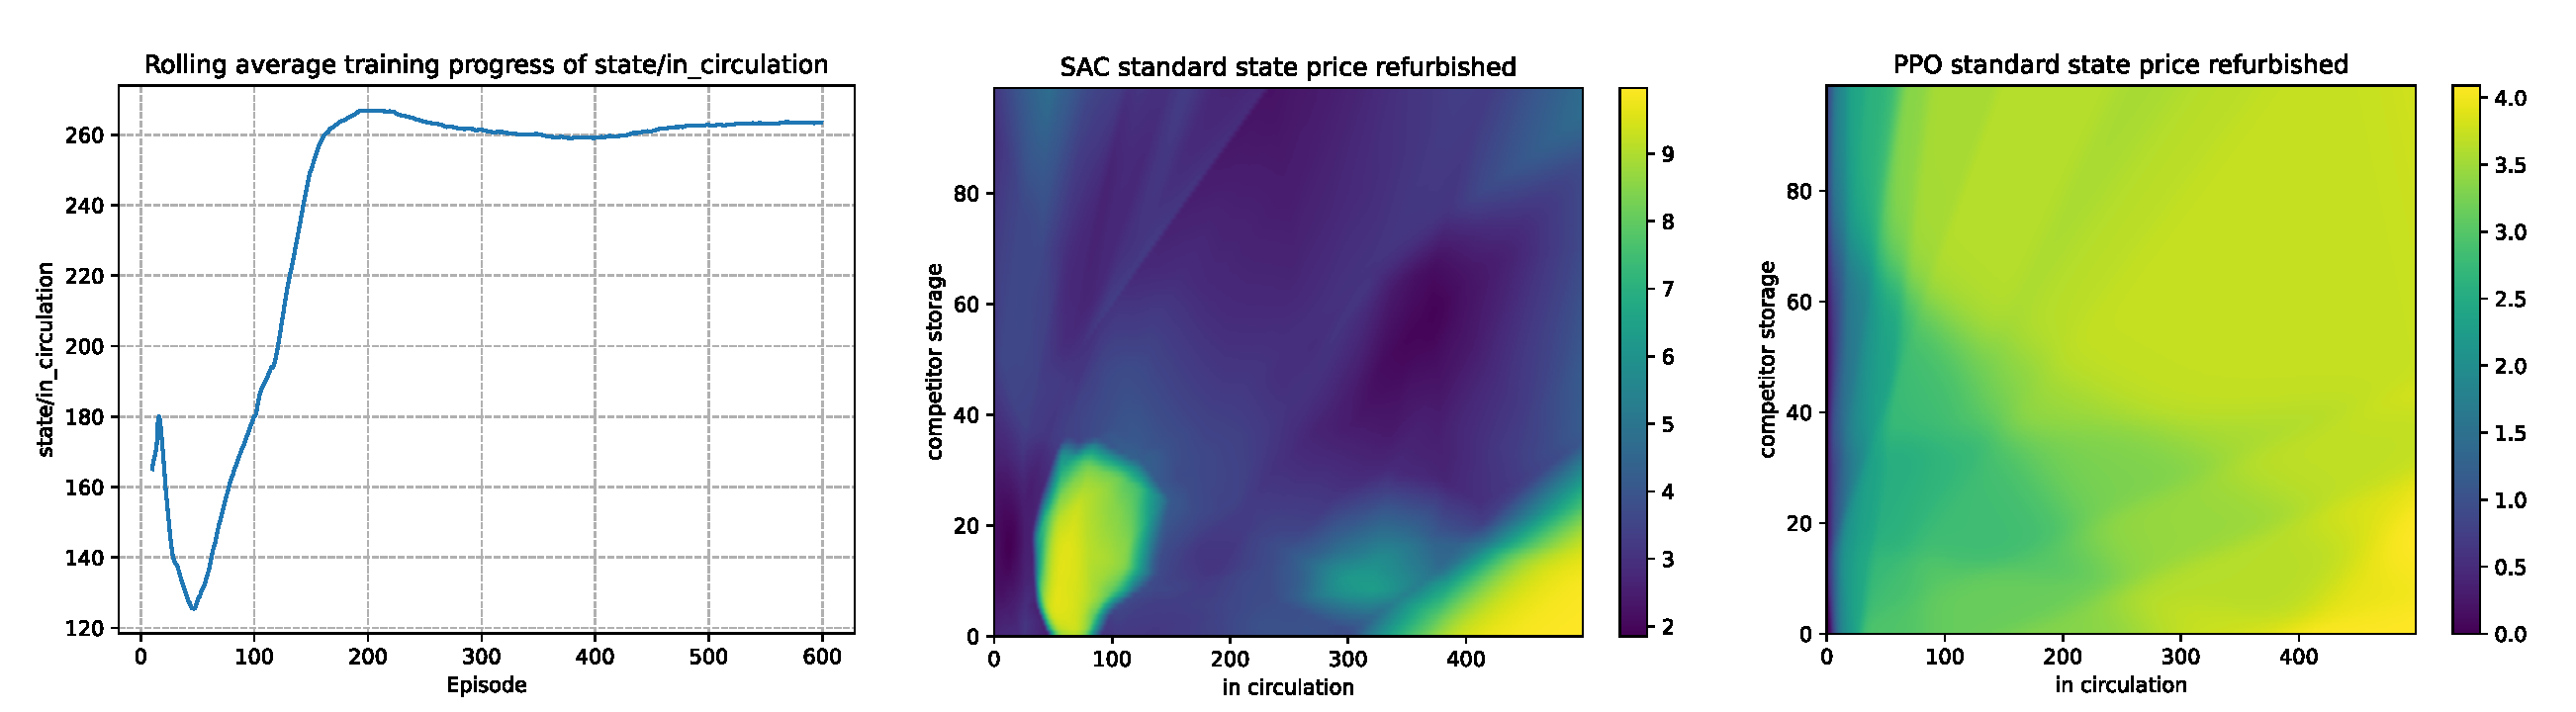
\includegraphics[width=\textwidth]{main/sac_in_circulation_dependend_explanation.pdf}
	\caption{Betrachtung der Agenten mit vollständiger Information: (links) Verlauf des \textit{in-circulation}-Zählers im SAC-Training, (mittig und rechts) Gebrauchtpreis in Abhängigkeit von \textit{in-circulation} und Lagerstand des Konkurrenten bei SAC und PPO; andere Argumente sind dabei fest auf einen Wert gewählt, der typisch bei einem Trainingsdurchlauf ist (eigener Lagerstand: 25, Neupreis Konkurrent: 6, Gebrauchtpreis Konkurrent: 4, Rückkaufpreis Konkurrent: 0)}
	\label{graphic:InCirculationExplain}
\end{figure}
Für das spezielle Phänomen bei SAC drängt sich aber noch ein weiterer Erklärungsansatz auf.
Zunächst kann aus Abbildung \ref{graphic:InCirculationExplain} (Mitte) gelesen werden, dass der SAC-Agent Abhängigkeiten der beiden Argumente (Zähler der Anzahl in Zirkulation und Lagerstand des Konkurrenten) erlernt.
Dass sich eine nahezu optimale Policy so verhalten sollte, ist angesichts der geringen Bedeutung der beiden Argumente auszuschließen, was die Policy des deutlich erfolgreicheren PPO-Agenten bestätigt.
Wie man es erwarten würde, hängt sie kaum von diesen beiden Argumenten ab.
Die niedrigere Spitzenperformance von SAC lässt sich (mindestens teilweise) durch diese Eigenschaften der Policy erklären.
Für die von SAC erlernte Policy lässt sich eine Erklärung in der Funktionsweise von Soft Actor Critic finden.
Sie basiert darauf, dass bei weiterentwickelten Policies im Markt mehr Produkte in Zirkulation sind.
Das ist in Abbildung \ref{graphic:InCirculationExplain} (links) gezeigt und liegt daran, dass wenig trainierte Policies im Gegensatz zu den weiterentwickelten oft zu viel zurückkaufen (und dabei zu viel Geld ausgeben).
Das bedeutet, dass gerade am Anfang der Experiencebuffer nur mit Zustandsübergänge mit niedrigen \textit{in-circulation}-Werten gefüllt wird.
Diese Samples bleiben im Experiencebuffer, sind aber für das spätere Training nicht mehr hilfreich und können die Anomalien in der Policy erklären.
So liegt eine starke Anomalie in der Policy im Bereich zwischen 50 und 150 Produkten in Zirkulation, genau der Bereich, aus dem die frühen Samples stammen.
Das Entfallen des \textit{in-circulation}-Eintrages verbessert also die Performance des SAC wohl deshalb, weil dieser dann nicht mehr die Möglichkeit hat, mit missweisenden Samples tatsächlich nicht existente Zusammenhänge zu erlernen.
Es ist damit als Schwäche von SAC gegenüber dem On-Policy-Verfahren PPO zu verzeichnen, dass es weniger gut in der Lage ist, die geringe Relevanz dieses Attributes selbstständig zu erlernen.